\documentclass[
  aspectratio=169,
]{beamer}

\usepackage[english]{babel}
\usepackage[utf8]{inputenc}
\usepackage[T1]{fontenc}
\usepackage{csquotes}
\usepackage{expl3,biblatex}
\addbibresource{crp.bib}
\usepackage{booktabs}
\usepackage{tikz}
\usetikzlibrary{positioning, arrows.meta, shapes.geometric, fit, backgrounds, calc}

\usetheme[
  workplace=fi,
]{MU}

% ── TikZ styles for the attention-block diagrams ─────────────────────────────
% Node names stay stable across slides — referenced on Concept and Rule slides.
\tikzset{
  op/.style    = {draw, rounded corners=2pt, minimum height=6mm, minimum width=14mm,
                  align=center, font=\scriptsize, fill=blue!8, inner sep=2pt},
  bilin/.style = {op, fill=red!12},                 % bilinear matmuls
  norm/.style  = {op, fill=green!12},               % LayerNorm / softmax
  add/.style   = {op, circle, minimum width=4mm, minimum height=4mm,
                  inner sep=0pt, fill=orange!20, font=\tiny},
  arrow/.style = {-{Latex[length=1.6mm]}, thick},
  ghost/.style = {draw=none, fill=none, font=\scriptsize\itshape, text=gray},
  rulebox/.style = {draw, dashed, rounded corners, inner sep=4pt, fill=yellow!10, font=\tiny},
}

% Acronyms and short commands. Vanilla LaTeX only — no amsmath/amssymb.
\newcommand{\eps}{\varepsilon}
\newcommand{\Rel}{\mathcal{R}}
\newcommand{\half}{\frac{1}{2}}
\newcommand{\reals}{\mathbf{R}}

\title[CRP for ViTs]{Concept Relevance Propagation for Vision Transformers}
\subtitle{Rules, canonizers, concepts}
\author[A.~Bajger]{Adam Bajger\texorpdfstring{\\}{, }RationAI lab}
\institute[FI MU]{Faculty of Informatics, Masaryk University}
\date{\today}
\subject{Explainable AI for Vision Transformers}
\keywords{LRP, AttnLRP, CRP, ViT, DINOv3, attention unfolding}

\begin{document}

% ─── Title ──────────────────────────────────────────────────────────────────
\begin{frame}[plain]
  \maketitle
\end{frame}

% ═══════════════════════════════════════════════════════════════════════════
\section[Motivation]{Motivation}
% ═══════════════════════════════════════════════════════════════════════════

\begin{frame}{Motivation}
ViTs dominate vision benchmarks. We want post-hoc explanations that are:
\begin{itemize}
  \item \alert{faithful} — the explanation conserves the predicted score,
  \item \alert{spatial} — pixel-level heatmaps,
  \item \alert{conceptual} — addressable per attention head, embedding
        dimension, and token position.
\end{itemize}
Plain gradient saliency violates conservation through softmax,
bilinear matmul, residual additions, and LayerScale: each is
non-linear in a way that the Jacobian does not faithfully unwind.

\smallskip
AttnLRP~\cite{achtibat2024attnlrp} introduces ViT-specific LRP rules
that recover conservation. CRP~\cite{achtibat2023crp} lifts attribution
from a single map per input to a map per \emph{concept}.

\smallskip
This talk: how to compose these rules through the \emph{two}
ViT block variants we work with (timm pre-norm and Eva/DINOv3) and
how to address concepts at the attention boundary.
\end{frame}

% ═══════════════════════════════════════════════════════════════════════════
\section[LRP]{LRP}
% ═══════════════════════════════════════════════════════════════════════════

\begin{frame}{LRP-0 and $\eps$-LRP}
\begin{block}{LRP-0 (Bach et al.\ 2015)}
For $y_j = \sum_i w_{ij}\, x_i + b_j$:
\[
  \Rel_i = \sum_j \frac{w_{ij}\, x_i}{\sum_k w_{kj}\, x_k}\, \Rel_j
\]
Exact conservation on linear layers.
\end{block}
\begin{block}{$\eps$-LRP (stabilised)}
\[
  \Rel_i = \sum_j \frac{w_{ij}\, x_i}{\eps\cdot \mathrm{sign}(z_j) + z_j}\, \Rel_j
\]
$\eps$ kills small-denominator amplification. Conservation $\sum \Rel_i \approx \sum \Rel_j$ within $\eps$.
\end{block}

\structure{Problem}: softmax, bilinear matmul, residual adds, LayerScale are NOT linear.
Stock LRP cannot route relevance through them.
\end{frame}

\begin{frame}{AttnLRP and our additions}
\textbf{AttnLRP}~\cite{achtibat2024attnlrp} adds per-non-linearity rules:
\begin{itemize}
  \item identity rule for softmax / LayerNorm / GELU (Eq.~9),
  \item bilinear rule for $Q K^\top$ and $\mathrm{attn} \cdot V$ (Prop.~3.3),
  \item std stop-gradient inside LayerNorm.
\end{itemize}

\textbf{Our additions} (detailed in the rule slides below):
\begin{itemize}
  \item \alert{AlphaBeta on bilinears} — Bach 2015's sign-split
        rule~\cite{bach2015lrp} generalised to bilinears, replacing
        AttnLRP's $2Y+\eps$ which inflates relevance at near-orthogonal
        $Q,K$ pairs.
  \item \alert{Magnitude-proportional residual split} — distributes
        relevance to skip and branch in proportion to their forward
        magnitudes; bounds the $2^L$ blow-up otherwise produced by an
        $L$-block residual chain.
  \item \alert{Uniform allocation on LayerScale} (AttnLRP Eq.~7
        applied to the LayerScale multiplier) — keeps relevance from
        decaying through small $\gamma$.
  \item \alert{Concept conditioning at the attention boundary} —
        mask the relevance tensor by head, embedding dim, or token
        position before the backward pass continues.
\end{itemize}
\end{frame}

% ═══════════════════════════════════════════════════════════════════════════
\section[Blocks]{ViT block variants}
% ═══════════════════════════════════════════════════════════════════════════

\begin{frame}{Two ViT block layouts}
\begin{columns}[T]
\begin{column}{0.48\textwidth}
\begin{exampleblock}{Standard timm ViT~\cite{dosovitskiy2021vit}}
Pre-norm, no RoPE, no LayerScale, 1 cls token.\\
$N = 1 + 196 = 197$ tokens.
\end{exampleblock}
\end{column}
\begin{column}{0.48\textwidth}
\begin{exampleblock}{Eva / DINOv3~\cite{darcet2024dinov3}}
Pre-norm, RoPE~\cite{su2021rope} on $Q/K$, LayerScale~\cite{touvron2021cait} $\gamma$, 4 register tokens prepended to cls.\\
$N = 5 + 256 = 261$ tokens.
\end{exampleblock}
\end{column}
\end{columns}

\vspace{4mm}
Both share the macro pipeline
\[
  \mathbf{x} \to \mathrm{LN} \to \mathrm{Attn} \to \mathrm{LayerScale}? \to \mathrm{add}_1 \to \mathrm{LN} \to \mathrm{MLP} \to \mathrm{LayerScale}? \to \mathrm{add}_2
\]
and differ only in the attention internals (next two slides).
\end{frame}

% ── Diagram A: standard timm ViT ──────────────────────────────────────────
\begin{frame}{Diagram A: timm ViT block}
\centering
\resizebox{0.98\textwidth}{!}{%
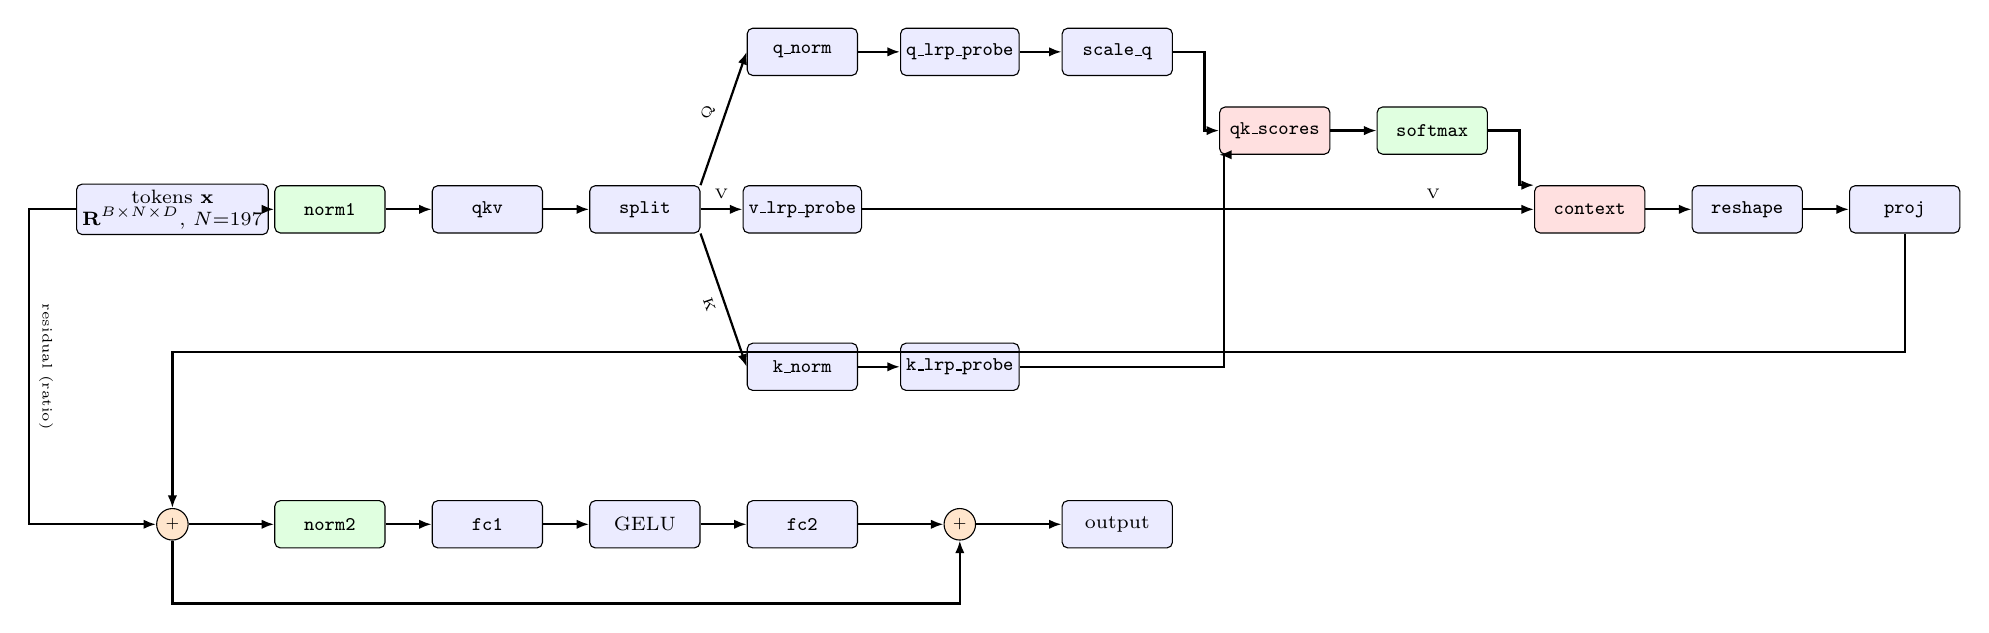
\begin{tikzpicture}[x=1cm, y=1cm]
  \node[op]    at ( 0,  0)   (xin)    {tokens $\mathbf{x}$ \\ \scriptsize$\reals^{B\times N\times D}$, $N{=}197$};
  \node[norm]  at ( 2,  0)   (norm1)  {\texttt{norm1}};
  \node[op]    at ( 4,  0)   (qkv)    {\texttt{qkv}};
  \node[op]    at ( 6,  0)   (split)  {\texttt{split}};

  \node[op]    at ( 8,  2.0) (qnorm)  {\texttt{q\_norm}};
  \node[op]    at ( 8,  0)   (vp)     {\texttt{v\_lrp\_probe}};
  \node[op]    at ( 8, -2.0) (knorm)  {\texttt{k\_norm}};

  \node[op]    at (10,  2.0) (qp)     {\texttt{q\_lrp\_probe}};
  \node[op]    at (10, -2.0) (kp)     {\texttt{k\_lrp\_probe}};

  \node[op]    at (12,  2.0) (scaleq) {\texttt{scale\_q}};

  \node[bilin] at (14,  1.0) (qk)     {\texttt{qk\_scores}};
  \node[norm]  at (16,  1.0) (sm)     {\texttt{softmax}};
  \node[bilin] at (18,  0)   (ctx)    {\texttt{context}};
  \node[op]    at (20,  0)   (rs)     {\texttt{reshape}};
  \node[op]    at (22,  0)   (proj)   {\texttt{proj}};

  \node[add]   at ( 0, -4)   (add1)   {$+$};
  \node[norm]  at ( 2, -4)   (norm2)  {\texttt{norm2}};
  \node[op]    at ( 4, -4)   (fc1)    {\texttt{fc1}};
  \node[op]    at ( 6, -4)   (gelu)   {GELU};
  \node[op]    at ( 8, -4)   (fc2)    {\texttt{fc2}};
  \node[add]   at (10, -4)   (add2)   {$+$};
  \node[op]    at (12, -4)   (xout)   {output};

  \draw[arrow] (xin)   -- (norm1);
  \draw[arrow] (norm1) -- (qkv);
  \draw[arrow] (qkv)   -- (split);
  \draw[arrow] (split.north east) -- node[font=\tiny, sloped, above]{Q} (qnorm.west);
  \draw[arrow] (split) -- node[font=\tiny, above]{V} (vp);
  \draw[arrow] (split.south east) -- node[font=\tiny, sloped, below]{K} (knorm.west);
  \draw[arrow] (qnorm)  -- (qp);
  \draw[arrow] (qp)     -- (scaleq);
  \draw[arrow] (scaleq.east) -- ++(0.4,0) |- (qk.west);
  \draw[arrow] (knorm)  -- (kp);
  \draw[arrow] (kp.east) -- ++(2.6,0) |- (qk.south west);
  \draw[arrow] (qk)     -- (sm);
  \draw[arrow] (sm.east) -- ++(0.4,0) |- (ctx.north west);
  \draw[arrow] (vp.east) -- node[font=\tiny, above, pos=0.85]{V} (ctx.west);
  \draw[arrow] (ctx)    -- (rs);
  \draw[arrow] (rs)     -- (proj);
  \draw[arrow] (proj.south) -- ++(0,-1.5) -| (add1.north);
  \draw[arrow] (add1)   -- (norm2);
  \draw[arrow] (norm2)  -- (fc1);
  \draw[arrow] (fc1)    -- (gelu);
  \draw[arrow] (gelu)   -- (fc2);
  \draw[arrow] (fc2)    -- (add2);
  \draw[arrow] (add2)   -- (xout);
  \draw[arrow] (xin.west) -- ++(-0.6,0) |- node[font=\tiny, sloped, above, pos=0.25]{residual (ratio)} (add1.west);
  \draw[arrow] (add1.south) -- ++(0,-0.8) -| (add2.south);
\end{tikzpicture}%
}

\vspace{2mm}
\scriptsize Red nodes: bilinear matmuls ($Q K^\top$ and $\mathrm{attn}\cdot V$) — AlphaBeta rule.
Green nodes: normalisations — identity rule.
Blue nodes: linears ($Wx + b$) — $\eps$-LRP.
The \texttt{*\_lrp\_probe} nodes are identity placeholders on the
$Q$/$K$/$V$ paths after the qkv-split; they hold no parameters and
serve as named handles for concept conditioning at the attention boundary.
\end{frame}

% ── Diagram B: Eva / DINOv3 ────────────────────────────────────────────────
\begin{frame}{Diagram B: Eva / DINOv3 block}
\centering
\resizebox{0.98\textwidth}{!}{%
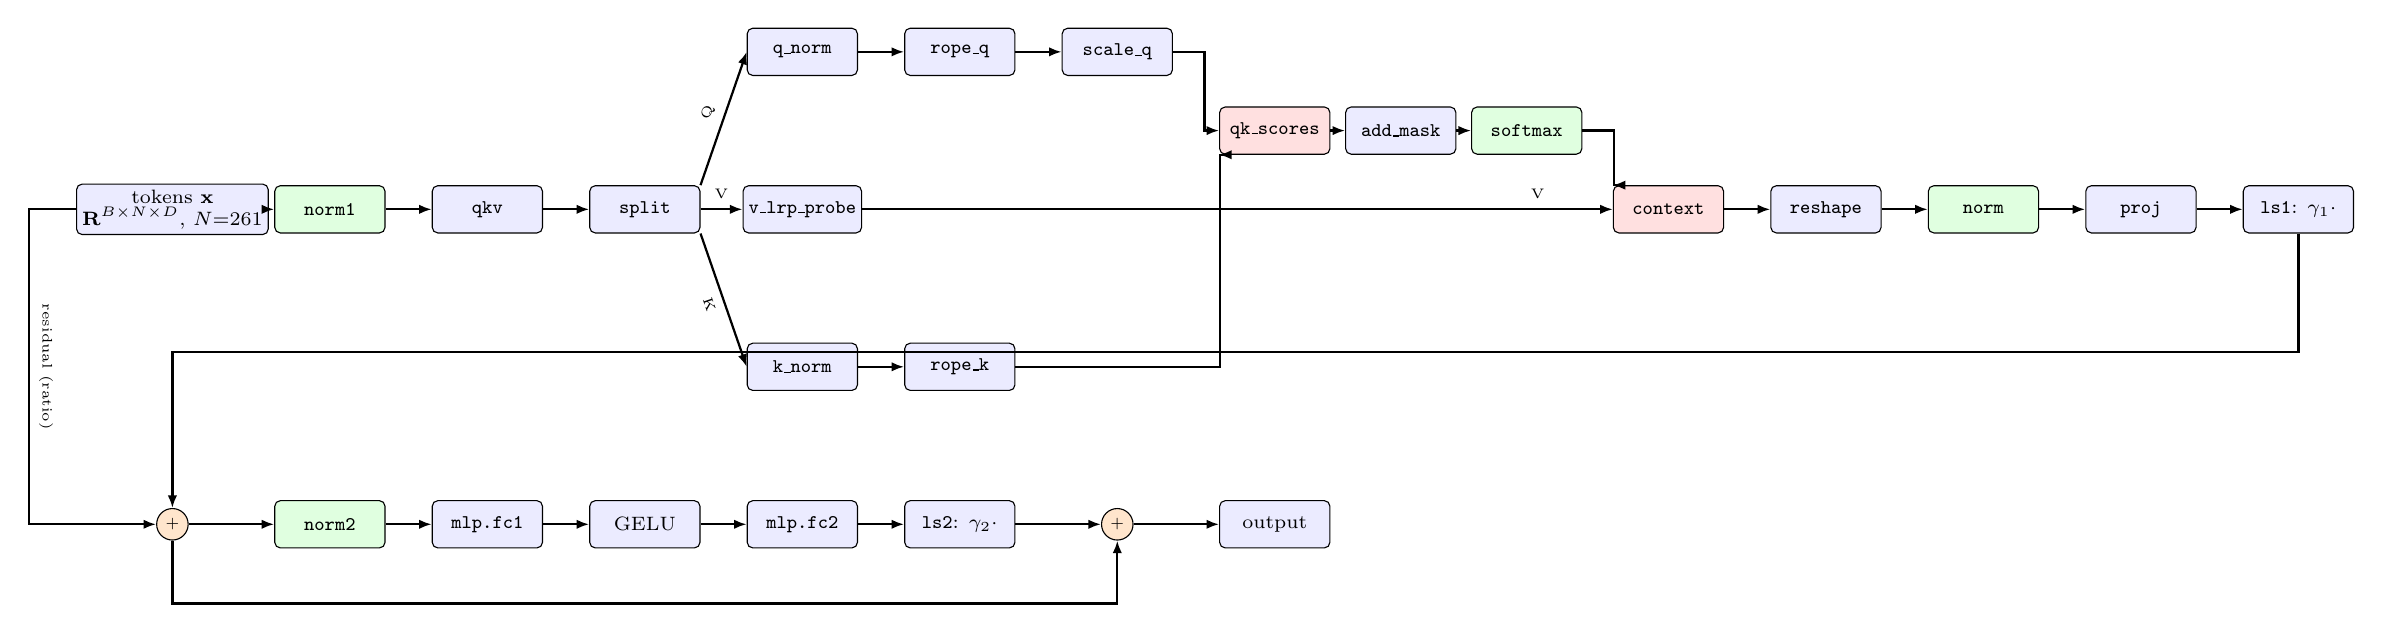
\begin{tikzpicture}[x=1cm, y=1cm]
  \node[op]    at ( 0,  0)    (xin)    {tokens $\mathbf{x}$ \\ \scriptsize$\reals^{B\times N\times D}$, $N{=}261$};
  \node[norm]  at ( 2,  0)    (norm1)  {\texttt{norm1}};
  \node[op]    at ( 4,  0)    (qkv)    {\texttt{qkv}};
  \node[op]    at ( 6,  0)    (split)  {\texttt{split}};

  \node[op]    at ( 8,  2.0)  (qnorm)  {\texttt{q\_norm}};
  \node[op]    at ( 8,  0)    (vp)     {\texttt{v\_lrp\_probe}};
  \node[op]    at ( 8, -2.0)  (knorm)  {\texttt{k\_norm}};

  \node[op]    at (10,  2.0)  (rq)     {\texttt{rope\_q}};
  \node[op]    at (10, -2.0)  (rk)     {\texttt{rope\_k}};

  \node[op]    at (12,  2.0)  (sq)     {\texttt{scale\_q}};

  \node[bilin] at (14,  1.0)  (qk)     {\texttt{qk\_scores}};
  \node[op]    at (15.6,1.0)  (mask)   {\texttt{add\_mask}};
  \node[norm]  at (17.2,1.0)  (sm)     {\texttt{softmax}};
  \node[bilin] at (19,  0)    (ctx)    {\texttt{context}};
  \node[op]    at (21,  0)    (rs)     {\texttt{reshape}};
  \node[norm]  at (23,  0)    (n)      {\texttt{norm}};
  \node[op]    at (25,  0)    (proj)   {\texttt{proj}};
  \node[op]    at (27,  0)    (ls1)    {\texttt{ls1}: $\gamma_1\cdot$};

  \node[add]   at ( 0, -4)    (add1)   {$+$};
  \node[norm]  at ( 2, -4)    (norm2)  {\texttt{norm2}};
  \node[op]    at ( 4, -4)    (fc1)    {\texttt{mlp.fc1}};
  \node[op]    at ( 6, -4)    (gelu)   {GELU};
  \node[op]    at ( 8, -4)    (fc2)    {\texttt{mlp.fc2}};
  \node[op]    at (10, -4)    (ls2)    {\texttt{ls2}: $\gamma_2\cdot$};
  \node[add]   at (12, -4)    (add2)   {$+$};
  \node[op]    at (14, -4)    (xout)   {output};

  \draw[arrow] (xin)   -- (norm1);
  \draw[arrow] (norm1) -- (qkv);
  \draw[arrow] (qkv)   -- (split);
  \draw[arrow] (split.north east) -- node[font=\tiny, sloped, above]{Q} (qnorm.west);
  \draw[arrow] (split) -- node[font=\tiny, above]{V} (vp);
  \draw[arrow] (split.south east) -- node[font=\tiny, sloped, below]{K} (knorm.west);
  \draw[arrow] (qnorm) -- (rq);
  \draw[arrow] (rq)    -- (sq);
  \draw[arrow] (sq.east) -- ++(0.4,0) |- (qk.west);
  \draw[arrow] (knorm) -- (rk);
  \draw[arrow] (rk.east) -- ++(2.6,0) |- (qk.south west);
  \draw[arrow] (qk)    -- (mask);
  \draw[arrow] (mask)  -- (sm);
  \draw[arrow] (sm.east) -- ++(0.4,0) |- (ctx.north west);
  \draw[arrow] (vp.east) -- node[font=\tiny, above, pos=0.9]{V} (ctx.west);
  \draw[arrow] (ctx)   -- (rs);
  \draw[arrow] (rs)    -- (n);
  \draw[arrow] (n)     -- (proj);
  \draw[arrow] (proj)  -- (ls1);
  \draw[arrow] (ls1.south) -- ++(0,-1.5) -| (add1.north);
  \draw[arrow] (add1)  -- (norm2);
  \draw[arrow] (norm2) -- (fc1);
  \draw[arrow] (fc1)   -- (gelu);
  \draw[arrow] (gelu)  -- (fc2);
  \draw[arrow] (fc2)   -- (ls2);
  \draw[arrow] (ls2)   -- (add2);
  \draw[arrow] (add2)  -- (xout);
  \draw[arrow] (xin.west) -- ++(-0.6,0) |- node[font=\tiny, sloped, above, pos=0.25]{residual (ratio)} (add1.west);
  \draw[arrow] (add1.south) -- ++(0,-0.8) -| (add2.south);
\end{tikzpicture}%
}

\vspace{2mm}
\scriptsize Adds \texttt{rope\_q}/\texttt{rope\_k} (RoPE on $Q$ and
$K$), \texttt{add\_mask}, a post-attention LayerNorm \texttt{norm},
and \texttt{ls1}/\texttt{ls2} (LayerScale $\gamma_1, \gamma_2$).
Otherwise identical structure and rule mapping to Diagram A.
\end{frame}

\begin{frame}{Attention unfolding}
Standard attention is one expression
\[
  \mathrm{Attn}(\mathbf{x}) \;=\; \mathrm{softmax}\!\left(\tfrac{Q K^\top}{\sqrt{d_h}}\right) V .
\]
The per-tensor LRP rules from the next section need a handle on each
constituent op: the bilinear $Q K^\top$, the softmax, and the bilinear
$\mathrm{attn}\cdot V$. \emph{Unfolding} is the algebraic rewrite of
the same forward as a composition of named ops:
\[
  Q K^\top \;\to\; \mathrm{add\ mask} \;\to\; \mathrm{softmax} \;\to\; (\cdot V) \;\to\; \mathrm{reshape} \;\to\; \mathrm{proj}.
\]
Forward output is bit-identical to the standard attention; what
changes is that each operation now has a named identity in the graph
where an LRP rule can attach and where a concept can be masked.

\smallskip
We also insert identity placeholders on the $Q$/$K$/$V$ paths right
after the \texttt{qkv}-split, so that any of our concepts can hook
into the per-head split before the reshape. Each of these four
hookable 3D sites carries the same shape
$\reals^{B\times N\times D}$ — a uniform contract that simplifies
concept design.
\end{frame}

% ═══════════════════════════════════════════════════════════════════════════
\section[Rules]{LRP rules}
% ═══════════════════════════════════════════════════════════════════════════

\begin{frame}{Rules — by operation type}
\small
\begin{tabular}{lll}
\toprule
Operation & Rule & Source \\
\midrule
Linear ($Wx + b$)                & $\eps$-LRP                  & \cite{bach2015lrp} \\
Element-wise nonlinearity        & Identity                    & AttnLRP Eq.~9~\cite{achtibat2024attnlrp} \\
Softmax (row-stochastic)         & Identity                    & AttnLRP Eq.~9~\cite{achtibat2024attnlrp} \\
LayerNorm                        & Identity, std stop-gradient & AttnLRP \S 3.2.2~\cite{achtibat2024attnlrp} \\
Constant scaling ($x \cdot c$)   & Identity                    & graph constant \\
Bilinear matmul ($A B$)          & AlphaBeta (sign-split)      & \cite{bach2015lrp} extended to bilinear \\
Residual addition ($x + b$)      & Magnitude-proportional split & this work \\
LayerScale ($\gamma \odot x$)    & Uniform allocation ($\half$) & AttnLRP Eq.~7~\cite{achtibat2024attnlrp} \\
\bottomrule
\end{tabular}

\vspace{4mm}
\centering Every rule below preserves LRP-0 conservation up to an $\eps$ residual.
\end{frame}

\begin{frame}{$\eps$-LRP}
For a pre-activation $z_j = \sum_i w_{ij}\, x_i + b_j$:
\[
  \Rel_i \;=\; \sum_j \frac{w_{ij}\, x_i}{\eps\cdot\mathrm{sign}(z_j) + z_j}\, \Rel_j .
\]

The numerator is the signed contribution of input $i$ to output $j$;
the denominator is the same as the forward pre-activation, regularised
by $\eps$ to bound the ratio when $|z_j|$ is small.

\smallskip
\textbf{Conservation.}
$\sum_i \Rel_i \;=\; \sum_j \Rel_j$ up to an $O(\eps)$ residual
(exact when $z_j$ is far from zero).

\smallskip
Applies to every linear projection in the ViT: \texttt{qkv}, attention
output projection, MLP \texttt{fc1}/\texttt{fc2}, classification head.
\end{frame}

\begin{frame}{Identity rule}
For an element-wise nonlinearity $y_i = f(x_i)$ the LRP-0 derivation
yields a one-to-one ratio that collapses to identity when $f$
contributed to the forward pass:
\[
  \Rel_i \;=\; \frac{y_i}{\eps\cdot\mathrm{sign}(y_i) + y_i}\, \Rel^{\mathrm{out}}_i
  \;\approx\; \Rel^{\mathrm{out}}_i \qquad (|y_i| \gg \eps).
\]
Conservation is exact ($\sum_i \Rel_i = \sum_i \Rel^{\mathrm{out}}_i$).

\smallskip
For \alert{softmax}: the row-stochastic property gives the same
collapse \cite{achtibat2024attnlrp} — relevance flows straight
through the softmax without going through its Jacobian, which would
otherwise mix relevance between query rows.

\smallskip
For \alert{LayerNorm}: treat $\sigma(x)$ as a graph constant
(stop-gradient). Then $y = \gamma\,(x-\mu)/\sigma + \beta$ is linear
in $x$ and the identity collapse applies to its element-wise affine
component \cite{achtibat2024attnlrp}.
\end{frame}

\begin{frame}{Bilinear rule: AlphaBeta on $A B$}
Standard bilinear rule (AttnLRP Prop.~3.3,~\cite{achtibat2024attnlrp})
divides by $2Y_{ij} + \eps$. Near-orthogonal $Q,K$ produce $Y_{ij}
\approx 0$ from \emph{cancellation} of large opposite-sign terms,
inflating each relevance contribution by $\sim 1/\eps$. We generalise
Bach's AlphaBeta rule~\cite{bach2015lrp} from linears to bilinears
to avoid this Case-B pathology structurally.

Sign-decompose: $A^\pm = \max/\min(A, 0)$, $B^\pm = \max/\min(B, 0)$.
The forward output splits into a purely-positive part and a
purely-negative part:
\[
  Y^+_{ij} = (A^+B^+ + A^-B^-)_{ij} \geq 0, \qquad
  Y^-_{ij} = (A^+B^- + A^-B^+)_{ij} \leq 0 .
\]
With $F = \Rel_Y / (Y^+ + \eps)$ and $G = \Rel_Y / (Y^- - \eps)$,
\[
  \Rel_A = \half \!\Bigl\{ A^+ \odot \bigl[\alpha (F B^{+\top}) + \beta (G B^{-\top})\bigr]
                          + A^- \odot \bigl[\alpha (F B^{-\top}) + \beta (G B^{+\top})\bigr] \Bigr\}
\]
(symmetric for $\Rel_B$; $\odot$ is the Hadamard product).

\smallskip
\textbf{Conservation.} $\sum \Rel_A + \sum \Rel_B = (\alpha+\beta)\sum \Rel_Y$ — exact when $\alpha+\beta=1$.
We choose $\alpha=\beta=\half$: balanced and structurally bounds
$|R_Y/Y^\pm|$ since the denominators cannot cancel internally.
\end{frame}

\begin{frame}{Residual rule: magnitude-proportional split}
A residual addition $y = x + \mathrm{branch}$ is bilinear in the two
operands' contributions. The unconditioned gradient sends the full
$\Rel_y$ down \emph{both} paths
($\Rel_x = \Rel_{\mathrm{branch}} = \Rel_y$), giving
$\sum\!\Rel = 2\sum\!\Rel_y$ per block and a $2^{L}$-fold blow-up
over an $L$-block stack.

We split $\Rel_y$ between $x$ and $\mathrm{branch}$ in proportion to
their (absolute) forward magnitudes:
\[
  \Rel_x \;=\; \Rel_y \odot \frac{|x|}{|x| + |\mathrm{branch}| + \eps},
  \qquad
  \Rel_{\mathrm{branch}} \;=\; \Rel_y \odot \frac{|\mathrm{branch}|}{|x| + |\mathrm{branch}| + \eps}.
\]
\smallskip
\textbf{Conservation.} $\Rel_x + \Rel_{\mathrm{branch}} = \Rel_y \cdot
(|x| + |\mathrm{branch}|)/(|x| + |\mathrm{branch}| + \eps) \to \Rel_y$
as $\eps \to 0$.

\smallskip
This generalises the LRP-0 \emph{contribution-proportional} principle
from a linear pre-activation to a sum of two non-additive operand
contributions. The signal that carried more magnitude through the
forward pass receives proportionally more relevance.
\end{frame}

\begin{frame}{LayerScale: uniform $\half$ allocation}
LayerScale~\cite{touvron2021cait}:
$\mathrm{branch} \to \gamma \odot \mathrm{branch}$ with a learned
per-channel $\gamma \in \reals^D$ initialised $\sim 10^{-4}$.

The naive Jacobian gives $\Rel_{\mathrm{branch}} = \gamma \odot \Rel_y$
— relevance decays geometrically by $\gamma$ at every LayerScale,
to $\sim 10^{-200}$ after a 24-block stack.

AttnLRP Eq.~7~\cite{achtibat2024attnlrp} treats the multiplication
as a bilinear of two operand sources ($\mathrm{branch}$ and $\gamma$)
and distributes relevance uniformly between them:
\[
  \Rel_{\mathrm{branch}} \;=\; \half\, \Rel_y,
  \qquad \Rel_{\gamma} \;=\; \half\, \Rel_y\ \text{(absorbed at $\gamma$).}
\]
Conservation: $\Rel_{\mathrm{branch}} + \Rel_\gamma = \Rel_y$ exactly.
Replaces the $\times\gamma$ deflation with a constant $\times\half$
per LayerScale that does not decay with depth.
\end{frame}

% ═══════════════════════════════════════════════════════════════════════════
\section[Concepts]{Concepts}
% ═══════════════════════════════════════════════════════════════════════════

\begin{frame}{From LRP to CRP}
LRP yields a single relevance map for an input. CRP
\cite{achtibat2023crp} promotes attribution to per-concept maps by
\emph{conditioning the backward pass}.

\begin{block}{Concept = partition of a hidden tensor}
At a chosen layer $\ell$ with hidden tensor $H_\ell \in \reals^{B \times N \times D}$,
a concept $c$ is a partition of the index space $\{(n, d)\}$ into
named parts. To attribute concept part $p$, mask the relevance to keep
only indices in $p$:
\[
  \Rel'_\ell[n,d] \;=\; \mathbb{1}[(n,d) \in p] \cdot \Rel_\ell[n,d],
\]
then continue the backward pass with the rules from before.
\end{block}

We define three concepts at the attention boundary, each partitioning
$H_\ell$ along a different axis: head ($D / H$ block of dims), single
dim, or token position.
\end{frame}

\begin{frame}{HeadConcept — partition by attention head}
The embedding dimension $D$ splits into $H$ contiguous head slices of
size $d_h = D/H$. Reshape
$\Rel \in \reals^{N \times D} \to \reals^{N \times H \times d_h}$.

\begin{block}{Mask for head $h$}
\[
  \Rel'_{n, h', d} \;=\; \mathbb{1}[h' = h] \cdot \Rel_{n, h', d}
\]
\end{block}

\begin{block}{Per-head attribution score}
\[
  a_h \;=\; \sum_{n=0}^{N-1} \sum_{d=0}^{d_h - 1} \Rel_{n, h, d}.
\]
\end{block}

Answers ``which head carried prediction-relevant signal at this
layer?''. Backward then continues with the masked $\Rel'$, producing
a per-pixel heatmap attributable to head $h$ specifically.
\end{frame}

\begin{frame}{EmbeddingDimConcept — partition by single dimension}
One part per dimension of $D$; finer-grained than HeadConcept.

\begin{block}{Mask for a dim set $S \subseteq \{0,\ldots,D-1\}$}
\[
  \Rel'_{n, d} \;=\; \mathbb{1}[d \in S] \cdot \Rel_{n, d}
\]
\end{block}

\begin{block}{Per-dim attribution score}
\[
  a_d \;=\; \sum_{n=0}^{N-1} \Rel_{n, d}.
\]
\end{block}

Useful when the heads' subspaces are themselves heterogeneous, or
to identify a single embedding direction that carries the prediction.
\end{frame}

\begin{frame}{TokenConcept — partition by token position}
Partitions on the token axis $\{0, \ldots, N-1\}$.

\begin{block}{Mask for a token set $T \subseteq [0, N)$}
\[
  \Rel'_{n, d} \;=\; \mathbb{1}[n \in T] \cdot \Rel_{n, d}
\]
\end{block}

\begin{block}{Per-position attribution score}
\[
  a_n \;=\; \sum_{d=0}^{D-1} \Rel_{n, d}.
\]
\end{block}

Lets us address the cls token, the patch tokens, or (on DINOv3) any
of the 4 \emph{register tokens}~\cite{darcet2024dinov3} —
signal sinks that absorb non-localised relevance and must be
attributable separately from the cls token.
\end{frame}

% ═══════════════════════════════════════════════════════════════════════════
\section[Datasets]{Datasets and models}
% ═══════════════════════════════════════════════════════════════════════════

\begin{frame}{Datasets — ground truth for XAI evaluation}
\centering\small
\begin{tabular}{l p{0.42\textwidth} p{0.34\textwidth}}
\toprule
Dataset & Ground-truth structure & What it lets us check \\
\midrule
FunnyBirds~\cite{hesse2023funnybirds}
  & 50 procedural bird classes; per-pixel part segmentation
  & does the heatmap localise the parts that distinguish the class? \\
dSprites~\cite{higgins2017dsprites}
  & 6 disentangled latent factors (shape, scale, orientation, position)
  & does the heatmap track the pixels of the labelled factor? \\
ColoredMNIST~\cite{nam2020lff}
  & digit shape and class-correlated colour as competing predictors;
    colour↔digit correlation broken on the test split
  & does the heatmap point at the shortcut (colour) or the true
    feature (stroke geometry)? \\
\bottomrule
\end{tabular}

\vspace{2mm}
Each dataset exposes a different kind of ground truth — part masks,
disentangled factors, a known spurious correlation — so that an
attribution can be assessed against an external standard, not just
visual plausibility.
\end{frame}

\begin{frame}{Models}
\centering\small
\begin{tabular}{ll}
\toprule
Backbone & Architecture \\
\midrule
vit\_dinov3~\cite{darcet2024dinov3}\,/\,\cite{oquab2024dinov2} (ViT-L/16, 24 blocks)
  & Eva-style block: pre-norm, RoPE on $Q/K$, LayerScale, 1 cls + 4 register tokens \\
vit\_base~\cite{dosovitskiy2021vit} (ViT-B/16, 12 blocks)
  & timm standard: pre-norm, no RoPE, no LayerScale, 1 cls token \\
vit\_small (ViT-S/16, 12 blocks)
  & timm standard, smaller embedding dim — same block layout as vit\_base \\
\bottomrule
\end{tabular}

\vspace{4mm}
Two block layouts → two unfolded substitutions exposing the same set
of named tensor ops. The same composite of LRP rules applies to all
three backbones; per-architecture features (RoPE, LayerScale, register
tokens) are handled by rules introduced above.
\end{frame}

% ═══════════════════════════════════════════════════════════════════════════
\section[Baselines]{Comparison baselines}
% ═══════════════════════════════════════════════════════════════════════════

\begin{frame}{Comparison baselines}
Two attention-attribution methods from the literature, evaluated on
the same images and the same models, for cross-comparison with the
LRP-based attributions.

Both methods hook the post-softmax attention weight tensor
$A^{(\ell)} \in \reals^{H \times N \times N}$ at each block $\ell$,
take $\partial y / \partial A^{(\ell)}$ by autograd, and produce the
shared per-block per-head quantity
\[
  M^{(\ell)} \;=\; \mathrm{mean}_h\bigl[(\nabla\!_{\!A^{(\ell)}}\, y\,\odot\, A^{(\ell)})_+\bigr]
  \;\in\; \reals^{N \times N}.
\]
They differ only in how $M^{(\ell)}$ across blocks is aggregated:

\begin{block}{LeGrad~\cite{bousselham2024legrad}}
\[
  \mathrm{heatmap} \;=\; \sum_{\ell \in \mathit{target}} \bigl[M^{(\ell)}\bigr]_{\,\mathrm{cls\ row},\,\mathrm{patch\ cols}}
\]
\end{block}

\begin{block}{Chefer's rollout~\cite{chefer2021transformer}}
\[
  R_0 = I,\qquad R_\ell \;=\; R_{\ell-1} + M^{(\ell)}\, R_{\ell-1}; \qquad \mathrm{heatmap} = [R_L]_{\,\mathrm{cls},\,\mathrm{patches}}
\]
\end{block}
\end{frame}

% ═══════════════════════════════════════════════════════════════════════════
\section{\bibname}
% ═══════════════════════════════════════════════════════════════════════════
\begin{frame}[t, allowframebreaks]{\bibname}
\printbibliography[heading=none]
\end{frame}

\begin{frame}[plain]
\begin{center}
\Huge Thank you for your attention.

\vspace{1cm}
\large Questions?
\end{center}
\end{frame}

\end{document}
